\chapter{Introduction}
\section{Basic Mathematical Models}
In this concise review we will provide brief explanations to the core concepts of differential equations, and include some examples to show the many techniques used in differential equations. Refer to the scratch paper if further examples and procedures are needed. For future reference the textbook used is "Elementary Differential Equations and Boundary Value Problems" by William E. Boyce and Richard C. DiPrima. All the graphics used in this document were created by Tarang Srivastava in Wolfram Mathematica \\

Equations considering derivatives are \textbf{differential equations}. A differential equation that describes a physical process is a \textbf{mathematical model}. \\
A model for an object falling in earth's atmosphere may be given by the differential equation $m \frac{dv}{dt} = mg - \gamma v$. Moving things around we get $\frac{dv}{dt} = 9.8 - \frac{v}{5}$ There are several solutions for this equation and can be represented by the slope field. \\
\begin{center}
	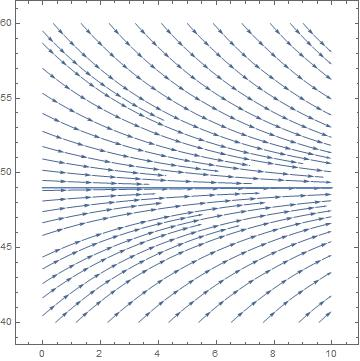
\includegraphics[width=7cm]{f1}
	$$\frac{dv}{dt} = 9.8 - \frac{v}{5}$$
\end{center}
The line $y=49$ shows the equilibrium solution for this case\\
\section{Solutions of Differential Equations}
When a problem is given where there are infinite solutions, usually when there is a constant in the solution as a result of integration, an \textbf{initial condition} can be set to find a particular answer, this is called an \textbf{initial value probelm}. A general example of this is
\begin{align*}
\dfrac{dy}{dt} = ay - b \\
y(0) = y_0 \\
\frac{dy/dt}{y-(b/a)} = a\\
\ln{ \vline y-(b/a) \vline} = at + C && \text{Where C is an arbitrary constant}\\ 
y = b/a + ce^{at} && \text{solve for C using the initial condition}\\
y = b/a + (y_0 - b/a)e^{at}
\end{align*}
The \textbf{general solution} with the constant gives all possible solutions, and graphs the \textbf{integral curves} 
\begin{center}
	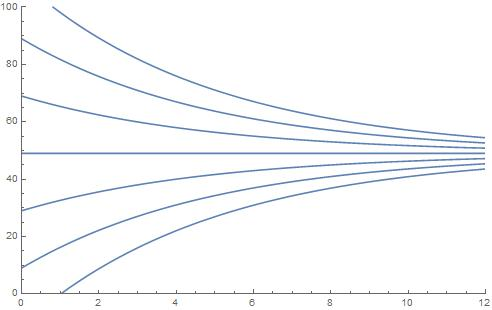
\includegraphics[width=12cm]{f2}
\end{center}
$$v = 49 + ce^{-t/5}$$
\section{Classification of Differential Equations}
Differential equations are classified into \textbf{ordinary differential equations} and \textbf{partial differential equations}. ODE have ordinary derivatives whereas PDE have partial derivatives. The \textbf{order} is the highest derivative. There are linear and nonlinear functions, we will mostly deal with linear for now. 
\pagebreak
\section{Chapter 1 Assessment}
\begin{multicols*}{2}
	\begin{enumerate}
		\item Consider the equation $\diff{p}{t} = 0.5p -450$ that gives the population of a certain species
		\begin{enumerate}
			\item Find the general solution to this equation
			\item Solve for the equilibrium solution 
			\item Solve for the specific solution if there are initially 1000 members in the species
		\end{enumerate}
		\item Consider the equation $\diff{y}{t} = ay - b$
		\begin{enumerate}
			\item Find the general solution
			\item Solve the initial value problem for $y(0) = y_0$
		\end{enumerate}
		\item Consider the equation $\diff{y}{t} + 2y = 3$ 
		\begin{enumerate}
			\item Find the integrating factor, $\mu(t)$ 
			\item Find the general solution 
			\item State the equilibrium solution 
		\end{enumerate}
		\item Show the solution for the arbitrary equation $\diff{y}{t} + ay = g(t)$ in terms of a general integral solution. 
		\item Solve the initial value problem for $ty' + 2y = 4t^2$ with the value $y(1) = 2$ 
		\item Solve the differential equation $\diff{y}{t} - 2y = 4 -t$, find the initial point that separates solutions that grow large positively to large negatively when $t\rightarrow \infty $ 
		\item Given the equation $\diff{p}{t} = 0.5p - 450$ that gives the population of a species (t = months)		\begin{enumerate}
			\item Find the time the population becomes extinct if $p(0) = 850$
			\item Find the time of extinction if $p(0) = p_0$ where $0 < p_0 < 900$
			\item Find the initial population if the population becomes extinct after 1 year 
		\end{enumerate}
	\end{enumerate}
\end{multicols*}